\section{Acquisto Hardware}
\labelsec{Hardware Procurement}

Sfortunatamente il primo problema incontrato in un progetto come il seguente e' stata la necessit\'a di acquistare la parte hardware del sistema che si andr\' a costruire. Di consequenza si e' messo in atto un processo di ricerca dei sensori, cavi e quant'altro per riuscire a soddisfare i requisiti

\subsection{Dispositivi di Computazione}

Prima di tutto necessitiamo di un dispositivo in grado di computare i dati emessi dai vari sensori e che sia interamente programmabile. Nel corso abbiamo visto due possibilita' che hanno avuto molto successo recentemente:

\begin{itemize}
  \item Arduino
  \item Raspberry Pi
\end{itemize}

Abbiamo scelto la seconda opzione data la maggior familiarita' con il dispositivo e dal momento in cui risulta piu' facile il riutilizzo dello stesso una volta terminato questo progetto.

\begin{figure}
	\centering
	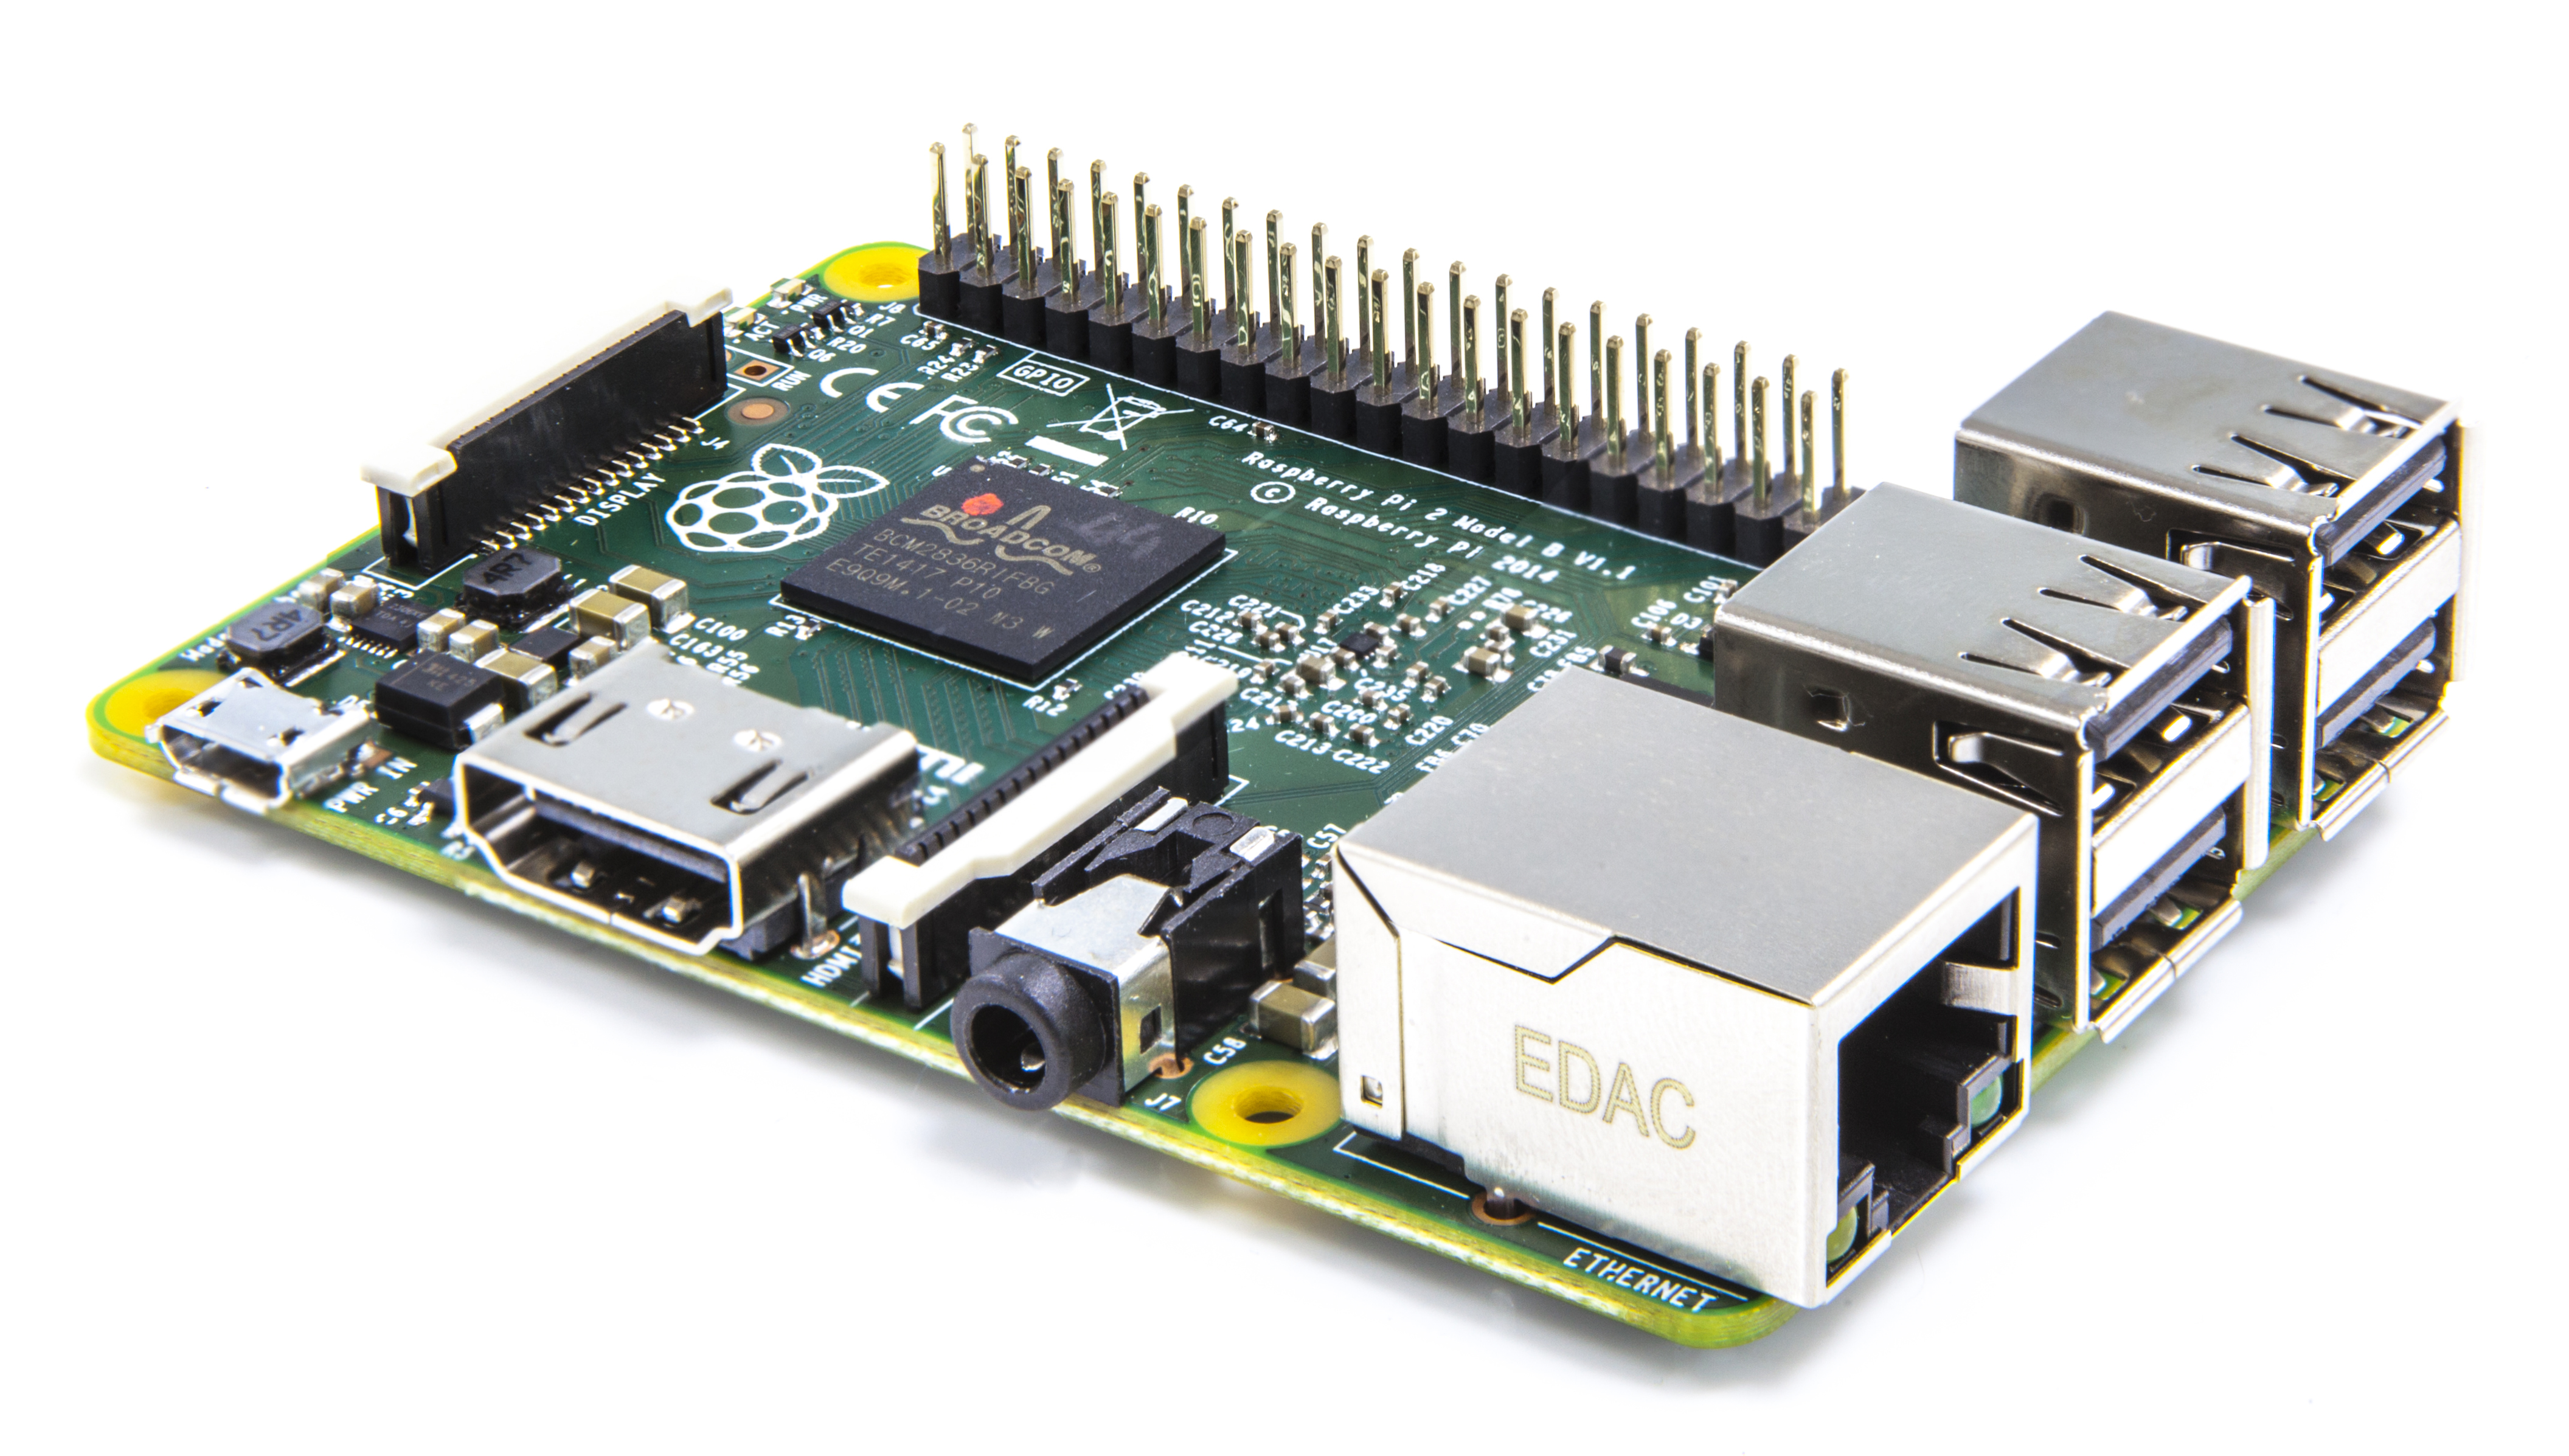
\includegraphics[width=0.7\linewidth]{Figures/Sensors&Rasp/Pi2}
	\caption[raspberry]{Scheda del Raspberry 2}
	\label{fig:Pi2}
\end{figure}



IIl Rasberry Pi 2 (figura~\ref{fig:Pi2}) è un SoC (sistema integrato) cio\'e possiede un chip che integra al suo interno processore, chipset, RAM ed eventuale circuteria input/output. \'E dotato delle seguenti uscite:

\begin{itemize}
	\item USB 2.0 (4)
	\item Ethernet
	\item HDMI
	\item Aux
	\item DC (Alimentazione)
	\item Slot MicroSD
\end{itemize}
Infine dispone di un GPIO (General Purpose Input/Output) interfaccia attraverso la quale è possibile comunicare con sensori esterni per mezzo di segnali digitali ed interagire con l'ambiente esterno.

Costo del dispositivo: 44,50 \euro


\subsection{Sensori}

Un'altra cosa fondamentale riguarda i sensori necessari per catturare i parametri richiesti.
Tutti i sensori per standard possono lavorare con una tensione di 5v.
Ogni sensore possiede 3 o 4 pin:

\begin{itemize}
	\item Vcc: Pin di alimentazione
	\item GND: Pin della massa
	\item Dout: Porta input/output digitale
	\item Aout: Porta input/output analogica (opzionale)
\end{itemize}

 Abbiamo Quindi scelto i sequenti sensori:

\begin{table}[]
	
	\begin{tabular}{lllll}
		\cline{1-3}
		\multicolumn{1}{|l|}{Parametri Ambientali} & \multicolumn{1}{l|}{Sensori} & \multicolumn{1}{l|}{Costo} &  &  \\ \cline{1-3}
		Temperatura \& Umidità                     & DHT11                        & 6\euro                          &  &  \\
		Luminosità                                 & Light                        & 5\euro                          &  &  \\
		Movimento                                  & HC-SR501                     & 6\euro                          &  &  \\
		Gas                                  & MQ-2                   & 7\euro                         &  &
	\end{tabular}
	\centering
	\caption{Sensor table}
	\label{my-label}

\end{table}


\newpage

\begin{figure}
\centering
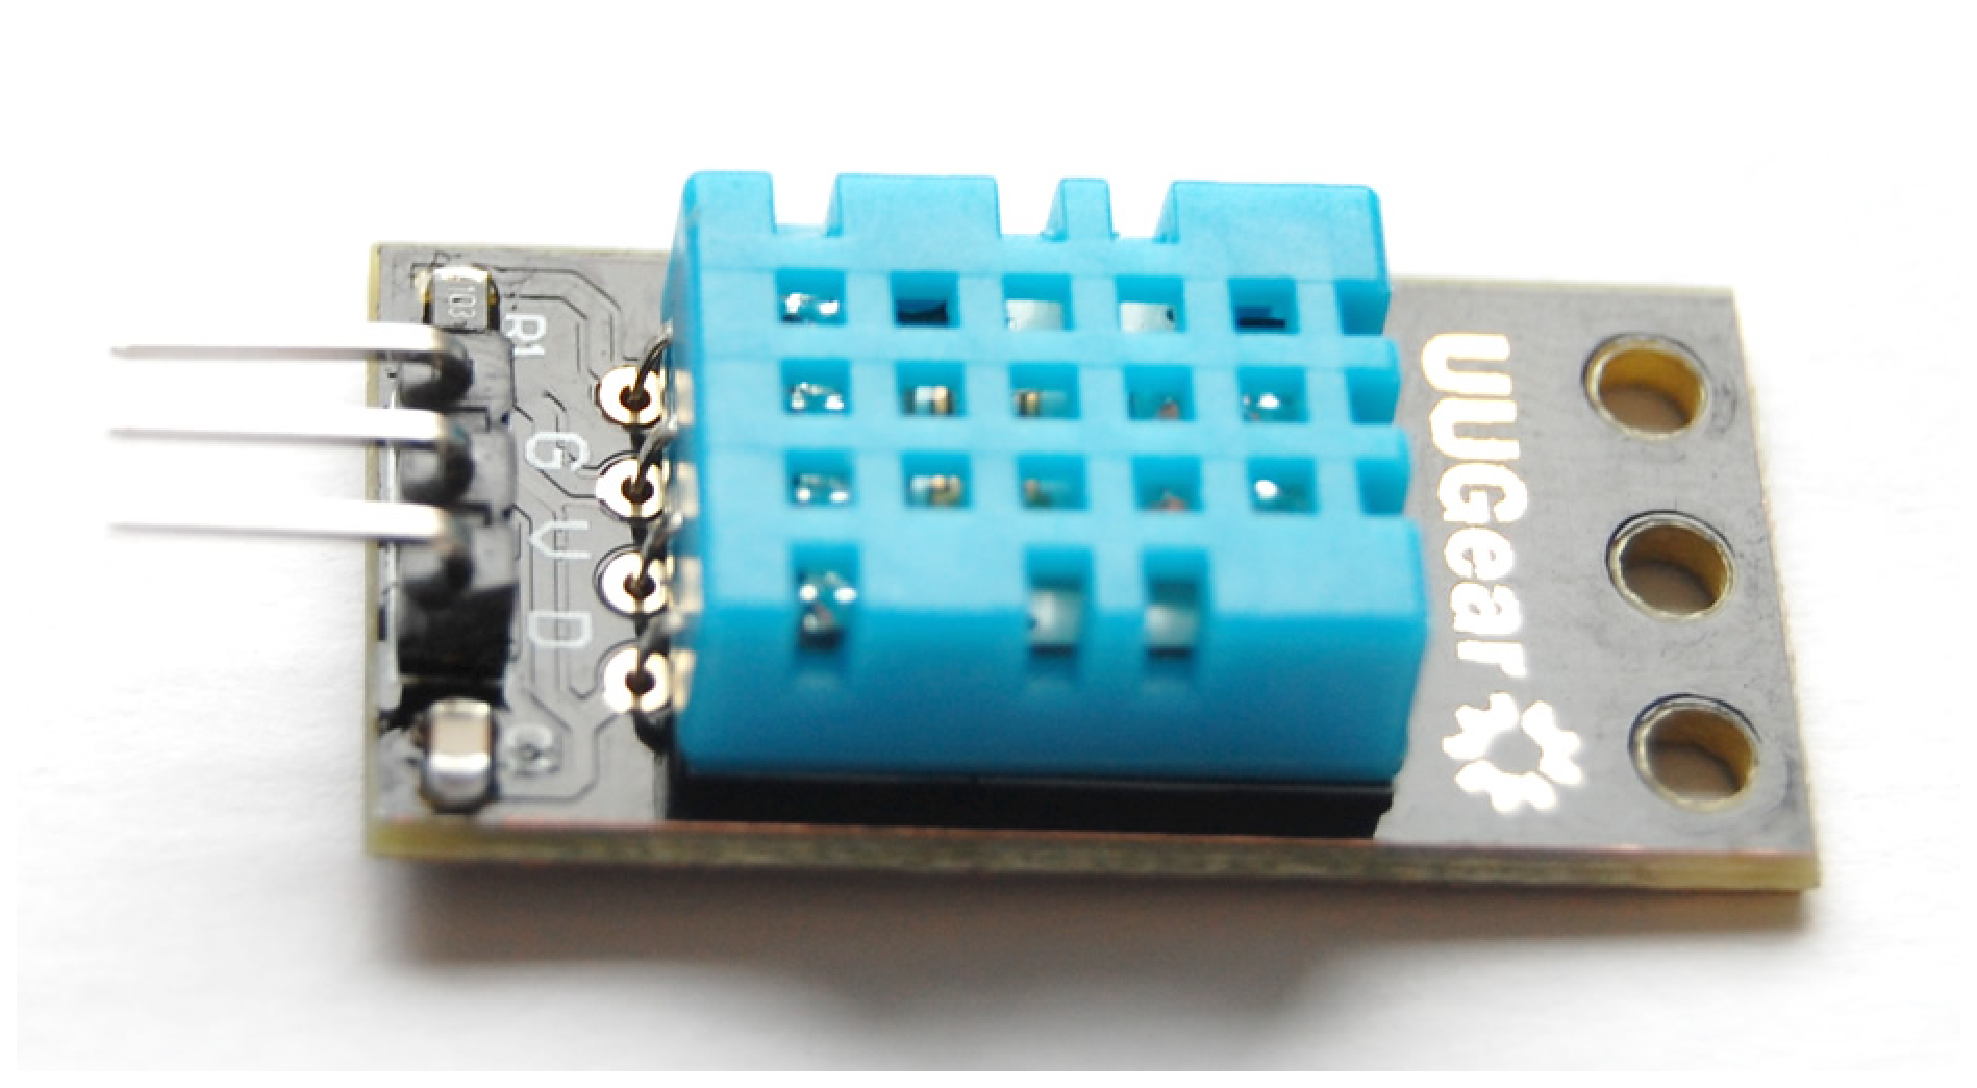
\includegraphics[width=0.7\linewidth]{Figures/Sensors&Rasp/dht11}
\caption[dht11]{DHT11 Sensor}
\label{fig:dht11}
\end{figure}

 Il sensore DHT11 (figura~\ref{fig:dht11}) è in grado rilevare la temperatura e l'umidità dell'ambiente circostante. Possiede 3 Pin per interfacciarsi.
 Le sue caratteristiche tecniche sono:
 
 \begin{itemize}
 	\item Vcc: 3.3$\sim$5.5V
 	\item Range: Temperatura 0 \textasciitilde 50℃, Umidità:  20-90%RH
 	\item Accuratezza: Temperatura +-2℃, Umidit\'a +-5%RH
 	\item Risoluzione: Temperatura  1℃, Umidit\'a  1%RH
 \end{itemize}
 
 \newpage
 
\begin{figure}
	\centering
	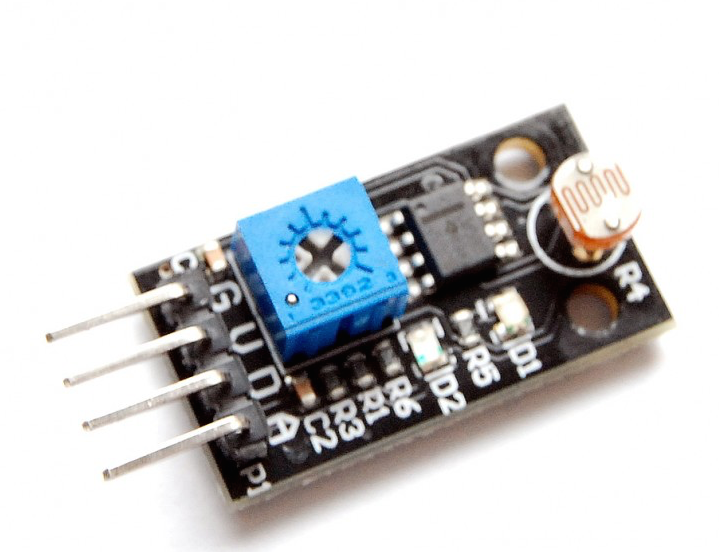
\includegraphics[width=0.7\linewidth]{Figures/Sensors&Rasp/light}
	\caption[light]{Light Sensor}
	\label{fig:light}

\end{figure}


Il sensore di luminosità (figura~\ref{fig:light} ) è un sensore dotato di un fotoresistore (componente circolare posizionato in fondo al circuito), un trimmer e due led. Il trimmer (equivalente ad un potenziometro) permette di regolare la sensibilità alla luce del sensore. Un led rimane costantemente acceso per indicare che il sensore è correttamente alimentato ed in funzione, l'altro si accende o si spegne nel momento in cui la luce percepita dal fotoresistore risulta sotto o sopra la soglia. Il sensore possiede 4 Pin per interfacciarsi.
Le sue caratteristiche tecniche sono:

\begin{itemize}
	\item Vcc: 3.3$\sim$5.5V
	\item Output: HIGH o LOW (boolean sensor: 0-1)
\end{itemize}

\newpage



\begin{figure}
	\centering
	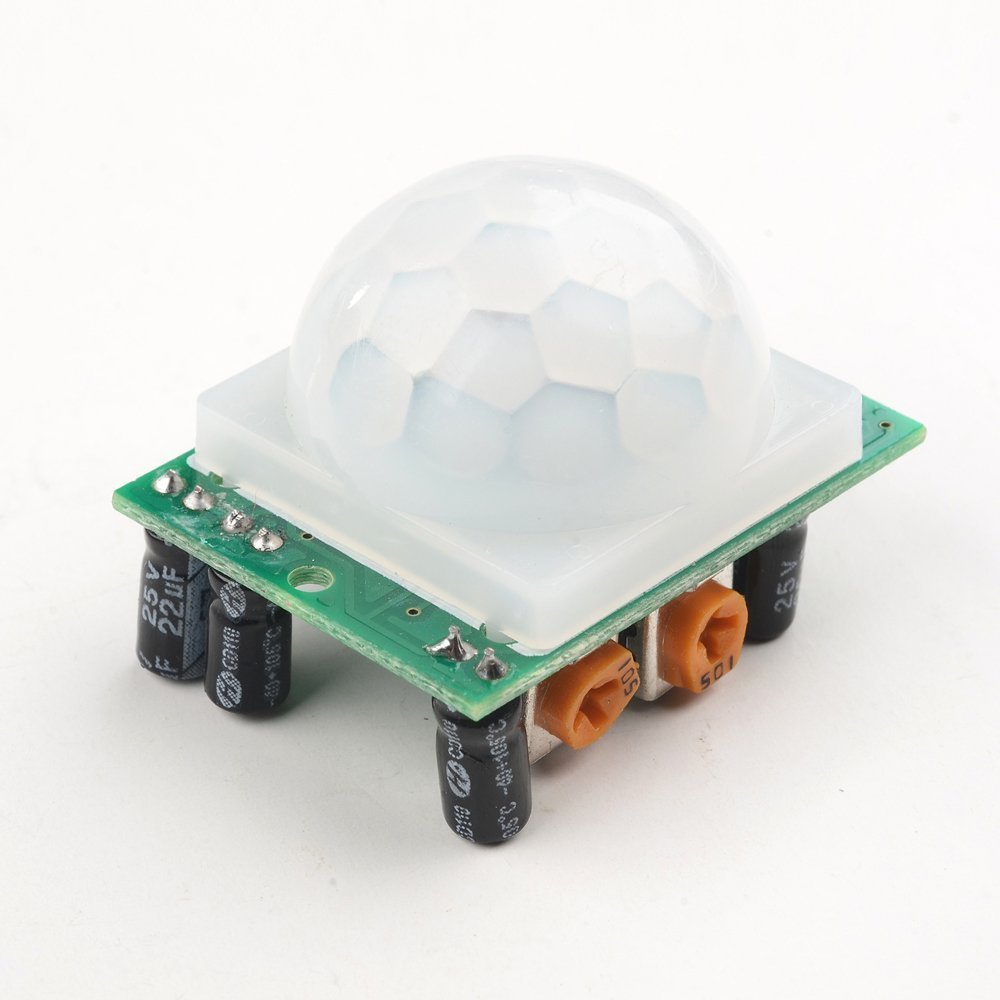
\includegraphics[width=0.7\linewidth]{Figures/Sensors&Rasp/pir}
	\caption[PIR] {HC-SR501 Sensor}
	\label{fig:pir}

\end{figure}



Il sensore di prossimità (figura~\ref{fig:pir}) permette di individuare gli spostamenti in una determinata area. Il suo funzionamento è dato da un componente chiamato "PIR" (Passive InfraRed) che per mezzo dei raggi infrarossi emanati dagli oggetti in uno spazio è in grado di percepire variazioni di movimento. Vi sono inoltre 2 trimmer arancioni per permettere di regolare il range di movimento e il tempo di delay. La semisfera di plastica trasparente posta sopra al modulo serve per poter massimizzare l'area di visibilità del sensore. Questa infatti, al suo interno, possiede particolari scanalature per che permettono di ridirigere correttamente i raggi al sensore. Vi sono 3 Pin per interfacciarsi.
Le sue caratteristiche tecniche sono:

\begin{itemize}
	\item Vcc: 5$\sim$20V
	\item Range: 5~7 metri
	\item Ampiezza: ~120°
	\item Tempo di delay : 0.3-600 secondi
	\item Output: HIGH o LOW (boolean sensor: 0-1)
\end{itemize}


\begin{figure}
	\centering
	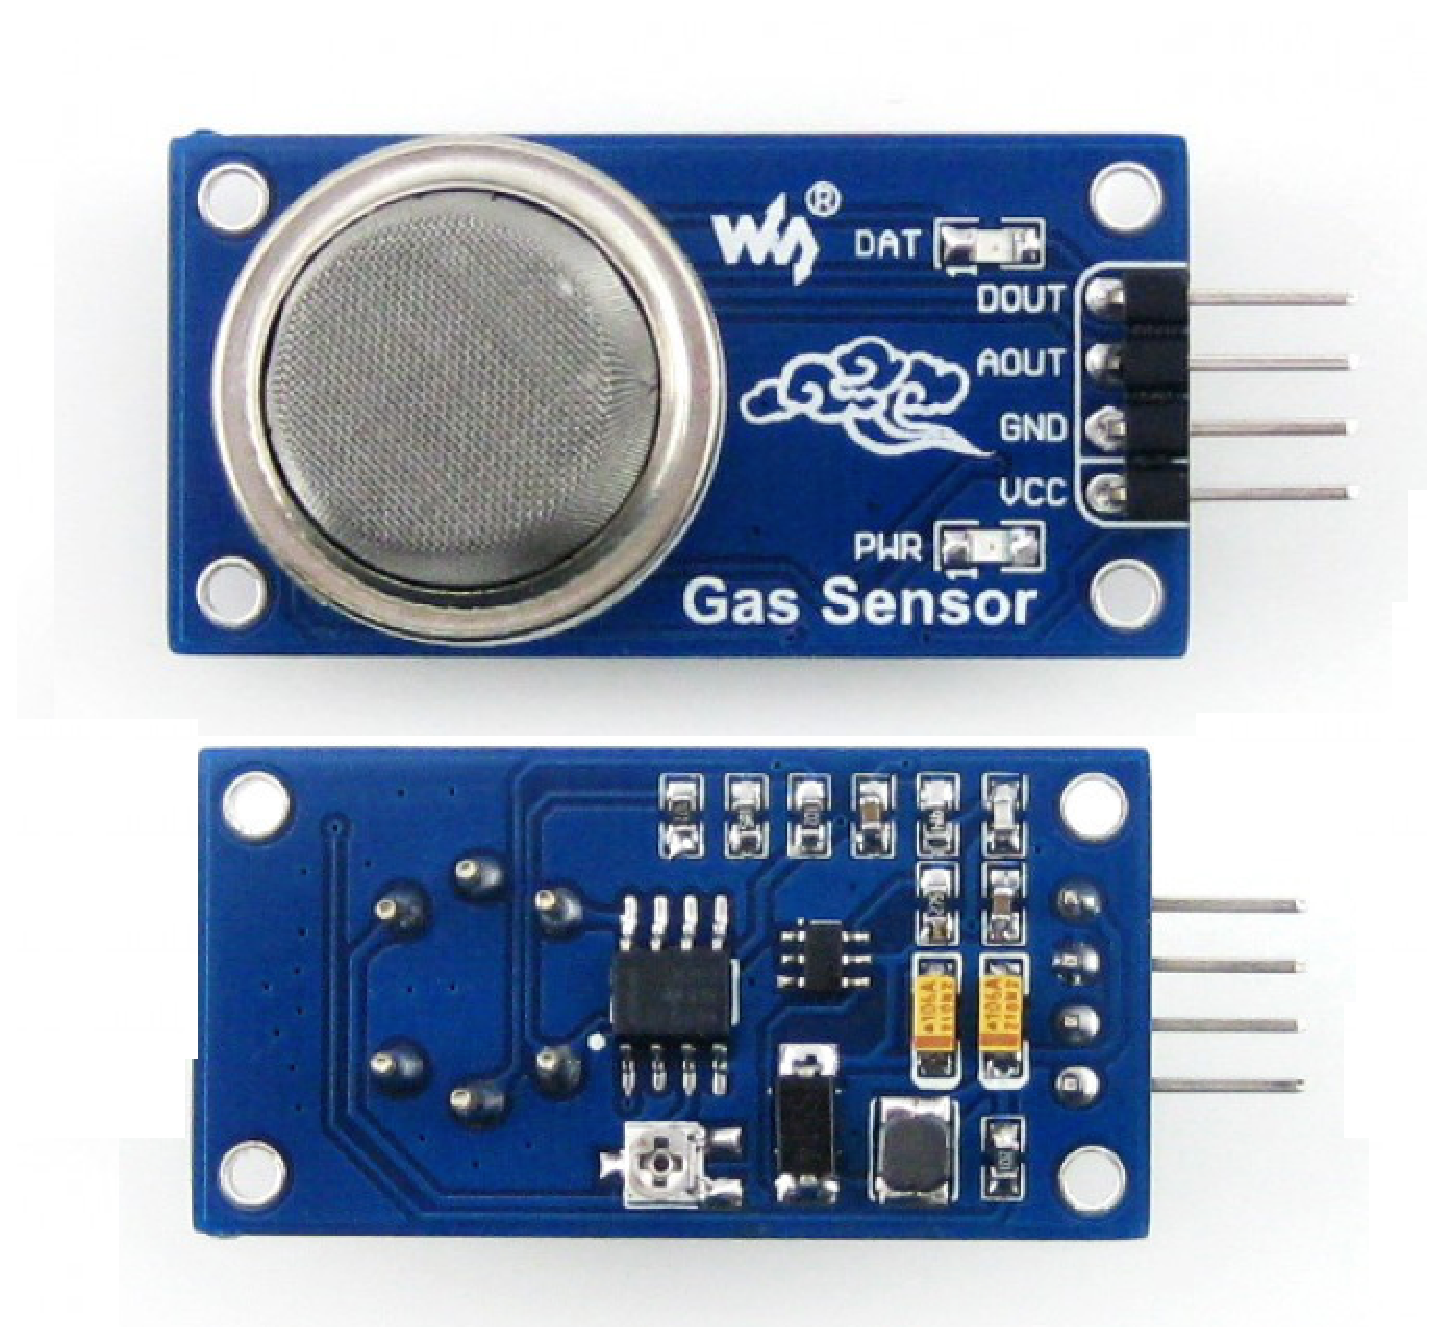
\includegraphics[width=0.7\linewidth]{Figures/Sensors&Rasp/mq-2}
	\caption[gas]{Gas sensor}
	\label{fig:mq2}

\end{figure}

Il sensore di gas (figura~\ref{fig:mq2}) è dotato di un sensore MQ-2 in grado di rilevare la presenza dei seguenti gas:  LPG, propano, idrogeno. Possiede inoltre due led: uno sempre acceso per segnalare la giusta alimentazione del sensore e l'altro per segnalare la presenza di gas (acceso quando vi è gas). Infine, sotto, vi è un trimmer utile alla regolazione della sensibilità del sensore. Vi sono 4 Pin per interfacciarsi.
Le sue caratteristiche tecniche sono: 

\begin{itemize}
	\item Vcc: 2,5$\sim$5V
	\item Output: HIGH o LOW (boolean sensor: 0-1)
\end{itemize}

\newpage



\subsection{Hardware Aggiuntivo}

Abbiamo cercato di realizzare il progetto provando a semplificare il più possibile la parte hardware.
In particolare ci siamo impegnati ad acquistare moduli (schede provviste di sensori e le resistenze necessarie al loro funzionamento) provvisti di sensore invece dei singoli sensori.

\begin{figure}
	\centering
	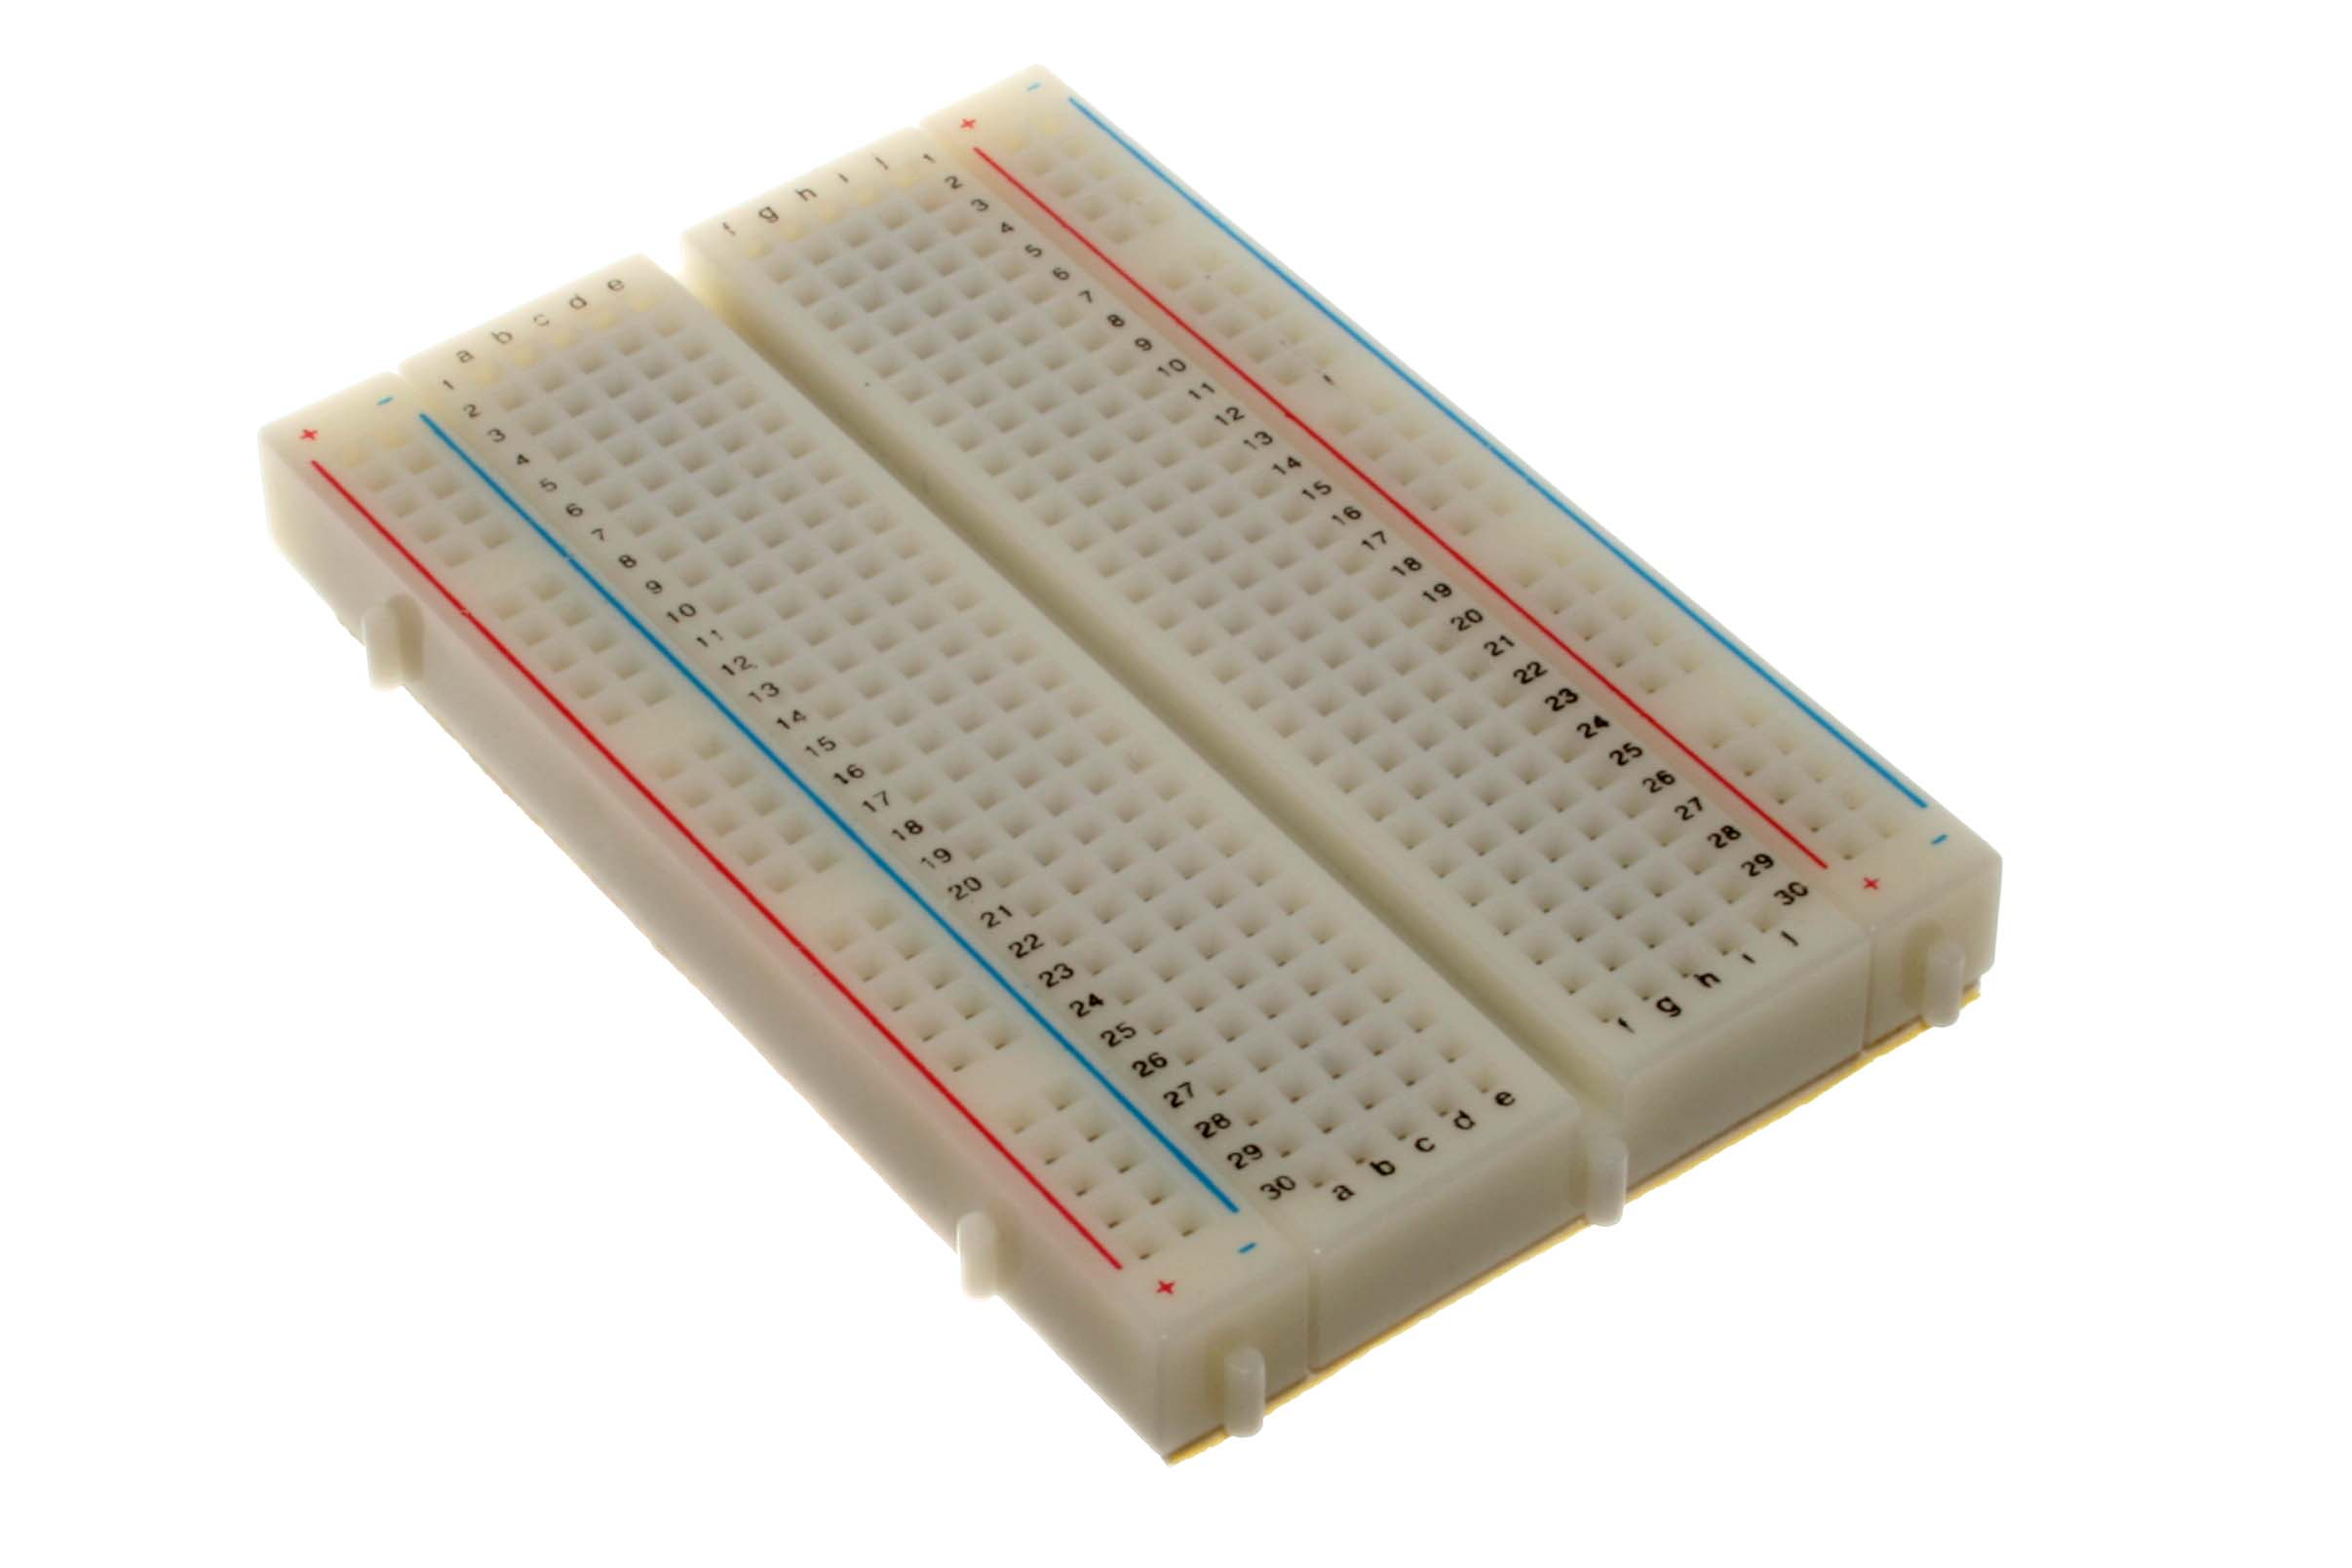
\includegraphics[width=0.7\linewidth]{Figures/Sensors&Rasp/breadboard}
	\caption[breadb]{Breadboard}
	\label{fig:bb}
	
\end{figure}

Questo ci ha permesso di fare a meno  resistenze, led o quant'altro che rendesse necessario l'uso della breadoard (figura~\ref{fig:bb}).
Strumento in grado di effettuare collegamenti, utilizzato molto spesso per realizzare e testare prototipi di circuiti elettrici.

\begin{figure}
	\centering
	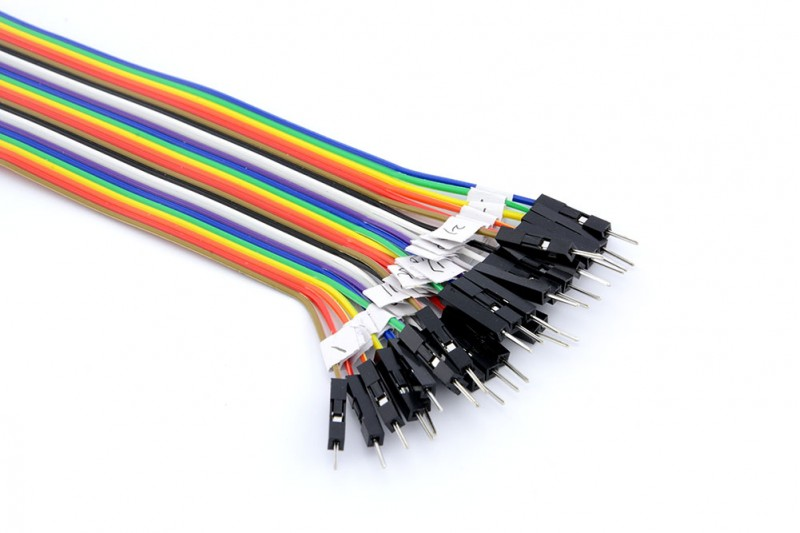
\includegraphics[width=0.7\linewidth]{Figures/Sensors&Rasp/cables}
	\caption[cable]{Cavi di collegamento}
	\label{fig:cables}
	
\end{figure}

\newpage

Tuttavia è stato necessario acquistare un set di cavi di collegamento (esempio in figura~\ref{fig:cables}), cioè cavi di metallo rivestiti in plastica, per permettere il collegamento dei vari pin dei sensori alla gpio del Rapberry.
	
Questi cavi possono essere di tre tipi a seconda delle combinazioni (maschio-maschio, maschio-femmina, femmina-femmina).

Il costo del set di cavi, composto da 50 cavi M-M , M-F, F-F è stato di 8€.

\newpage

